% !TEX encoding = UTF-8 Unicode
% !TEX spellcheck = de_DE
\documentclass[preprint]{vgtc}               % preprint

\ifpdf%                                % if we use pdflatex
  \pdfoutput=1\relax                   % create PDFs from pdfLaTeX
  \pdfcompresslevel=9                  % PDF Compression
  \pdfoptionpdfminorversion=7          % create PDF 1.7
  \ExecuteOptions{pdftex}
  \usepackage{graphicx}                % allow us to embed graphics files
  \DeclareGraphicsExtensions{.pdf,.png,.jpg,.jpeg} % for pdflatex we expect .pdf, .png, or .jpg files
\else%                                 % else we use pure latex
  \ExecuteOptions{dvips}
  \usepackage{graphicx}                % allow us to embed graphics files
  \DeclareGraphicsExtensions{.eps}     % for pure latex we expect eps files
\fi%

\graphicspath{{figures/}{pictures/}{images/}{./}} % where to search for the images





\usepackage{microtype}                 % use micro-typography (slightly more compact, better to read)
\usepackage[OT1]{fontenc}
\usepackage[utf8]{inputenc}
\PassOptionsToPackage{warn}{textcomp}  % to address font issues with \textrightarrow
\usepackage{textcomp}                  % use better special symbols
\usepackage{mathptmx}                  % use matching math font
\usepackage{times}
\usepackage[english,ngerman]{babel}                     
\renewcommand*\ttdefault{txtt}         % a nicer typewriter font
\usepackage{cite}                      % needed to automatically sort the references
\usepackage{tabu}                      % only used for the table example
\usepackage{booktabs}                  % only used for the table example
\usepackage{hyperref} 
%%%%%%%%%%%%%%%%%%%%%%%%%%%%%%%%%%%%%%%%%%%%%%%%%%%%%%%%%%%%%%%%%%%%%%%%%%%%%%%%%%%%%%%%%%%%%%%%%%%%%%%%%%%%%%%%%%%%%

\onlineid{0}

\vgtccategory{Research}

\vgtcinsertpkg

\preprinttext{Seminar Virtual und Augmented Reality -- WS 2019/20}

\title{Sensorisches Zusammenspiel des visuellen und vestibul\"aren Systems in Virtual Reality}

\author{Nils Henrik Seitz\thanks{e-mail: nils.seitz@uni-rostock.de}\\ \scriptsize Universit\"at Rostock}

\abstract{ Durch die zunehmende Digitalisierung der Gesellschaft, sinkende Kosten und gleichzeitig steigende Leistungsf\"ahigkeit der erfordlichen Hardware erfreut sich Virtual Reality immer gr\"oßerer Beliebtheit.
} 


\CCScatlist{ 
	\CCScat{H.1.2}{Models and Principles}{User/Machine Systems}{Human factors, Human information processing};
	\CCScat{H.5.1}{Information Interfaces and Presentation (e.g., HCI)}{Multimedia Information Systems}{Artificial, augmented, and virtual realities}
}

\keywords{Virtual Reality, Human Factors, Visual-Vestibular Conflict, Motion Sickness, Cyber Sickness}

% Make Structure(section, sub(sub)sections,
% figures and tables (LABEL THEM, do captions, width and centering)), <- AUTOREF
% make cites (FROM BIBDESK!!) 
%and footnotes, 
% sparsely use texttt / -it / -bf,
% enumerate/itemize (if necessary)
% use good latex math style (symbols, equtions, etc.) 

%% FIGURES
%\begin{figure}[tb]
%	\centering % avoid the use of \begin{center}...\end{center} and use \centering instead (more compact)
%	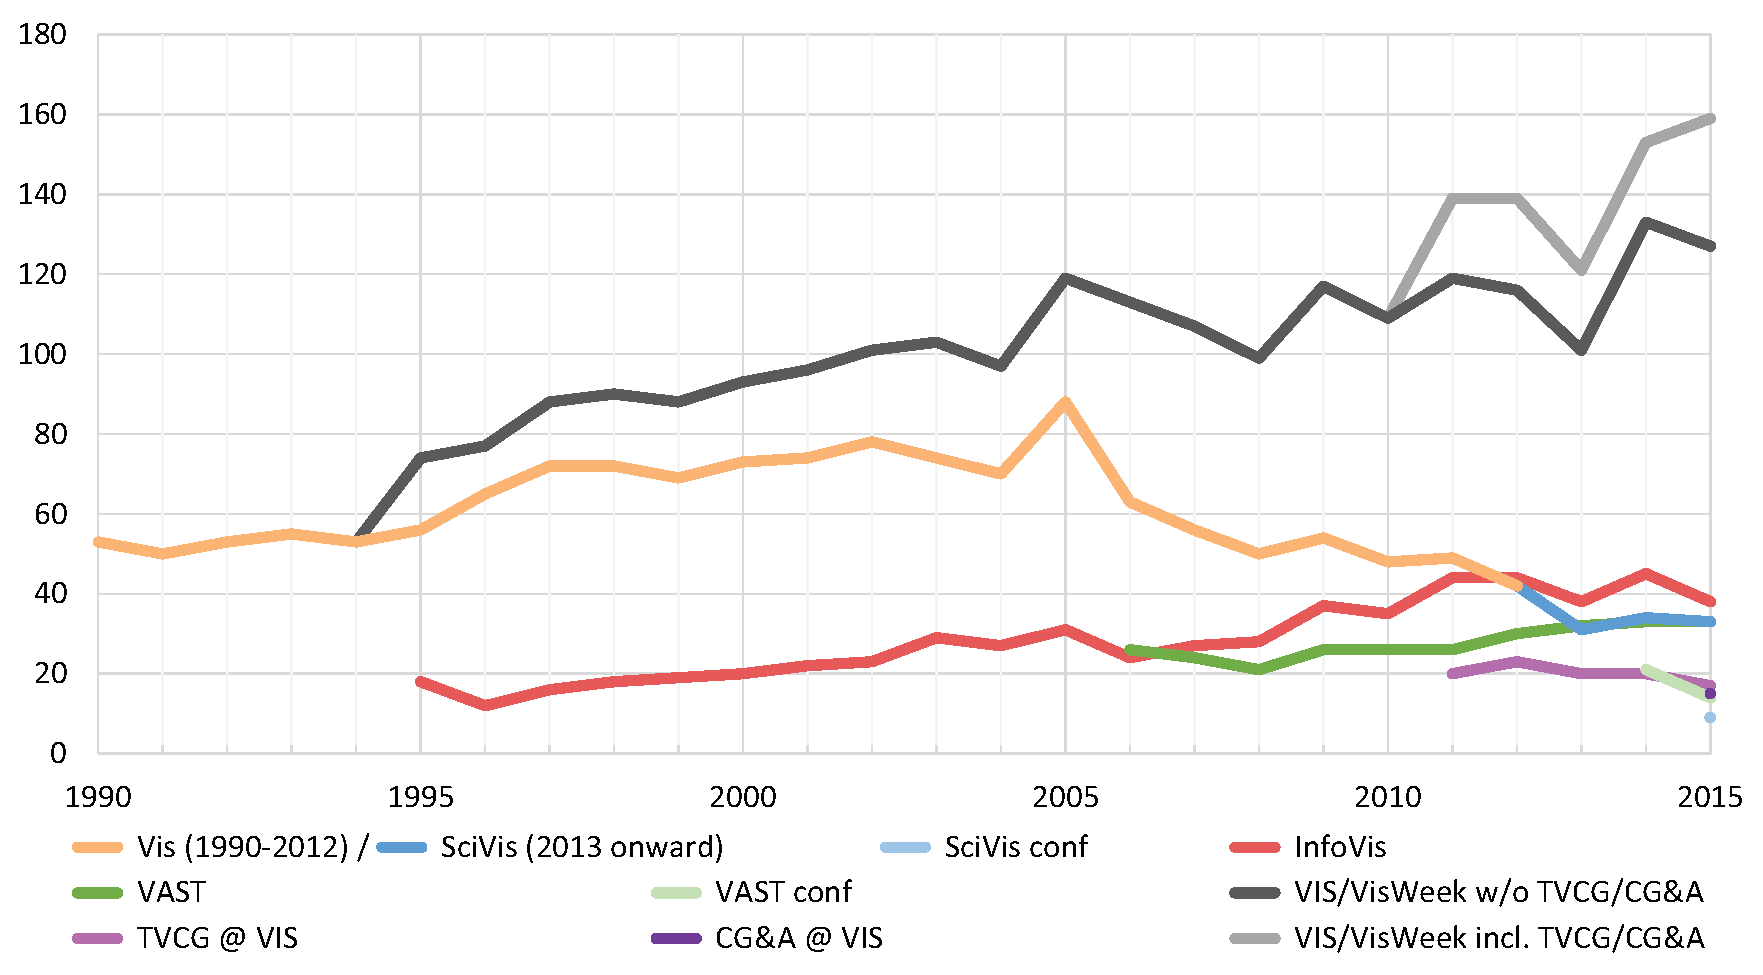
\includegraphics[width=\columnwidth]{paper-count-w-2015-new}
%	\caption{A visualization of the data from \autoref{tab:vis_papers}. The image is from \cite{Isenberg:2017:VMC} and is in the public domain.}
%	\label{fig:sample}
%\end{figure}

\begin{document}

\maketitle
\section{Einleitung} 
	Evolution\"ar gesehen, ist es die gr\"o{\ss}te St\"arke des Menschen, sich seiner Umgebung oder auch seine Umgebung an sich anzupassen. Daher liegt es in der Natur des Menschen, sich Werkzeuge herzustellen und Erfindungen zu machen, die im Alltag hilfreich sind.

Eine der wichtigsten Grundlagen daf\"ur ist die multisensorische Integration, ein evolution\"ares Wunder f\"ur sich, denn sie erm\"oglicht ein hohes, abstraktes Verst\"andnis und die F\"ahigkeit zu lernen. Unser Gehirn f\"uhrt unbemerkt und scheinbar m\"uhelos mehrmals innerhalb einer Sekunde die Informationen verschiedener Sinne zu einem f\"ur uns konsistenten Gesamtbild zusammen.
Dass diese Verarbeitung \"uberhaupt stattfindet, ist uns selten bewusst\cite{Deroy:2016:SensInte}. Sobald es dabei aber zu Komplikationen, das hei{\ss}t, Abweichungen der bisherigen Erfahrung, kommt, bemerken wir dies sofort. 

Eine relativ neue Erfindung ist Virtual Reality, mit der wir erstmalig die Chance haben, unsere Umgebung vollst\"andig nach unseren Vorstellung zu formen, beispielsweise auch mit ver\"anderten physikalischen Gesetzen.
Virtual Reality hat das enorme Potential, viele Bereiche der Gesellschaft nachhaltig zu ver\"andern, nur trifft es sich leider, dass genau bei der Integration der Sensorik Schwierigkeiten auftreten, die als Cyber Sickness bekannt sind.
	
\section{Motion Sickness und Cyber Sickness}
	In diesem Abschnitt sollen vorrangig grundlegende Arten von Motion Sickness erkl\"art und gegen\"uber gestellt sowie Theorien zur Entstehung dieser vorgestellt werden. Au{\ss}erdem soll darauf verwiesen werden, welche Probleme das f\"ur Virtual Reality impliziert.

Die gr\"o{\ss}ten Schwierigkeiten, die bei der Nutzung von Virtual Reality auftreten k\"onnen, sind die Symptome der Cyber Sickness. Diese \"ahneln denen der klassischen Motion Sickness und umfassen eine Vielzahl unangenehmer Empfindungen und Reaktionen durch den betroffenen Organismus: Kopfschmerzen, Schwei{\ss}ausbr\"uche, Orientierungslosigkeit, Schwindelanf\"alle, Ataxia und \"Ubelkeit bis hin zum Erbrechen\cite{LaViola:2000:CSinVR, Kolasinski:1998:SympCS}.

Durch die \"Ahnlichkeit in den k\"orperlichen Reaktionen zur klassischen Motion Sickness, die beispielsweise von Auto- oder Schifffahrten bekannt ist, versucht man auch, denselben Erkl\"arungsansatz zu verwenden: die \textit{Sensory Conflict Theory}\cite{Kolasinski:1998:SympCS,Johnson:2005:SCT_Expl}.
Diese postuliert, dass die eben genannten Symptome auftreten, wenn bei der multimodalen, sensorischen Integration\footnote{ Verarbeitung der Reize verschiedener Sinneskan\"ale auf h\"oheren kognitiven Ebenen} bez\"uglich der Selbstbewegung inkongruente Reize festgestellt wurden und intensiviert sich, wenn die aktuelle Wahrnehmung im Widerspruch mit vorherigen Lernerfahrung in \"ahnlichen Situationen steht\cite{Reason:1975:MSexp}.

Ein m\"oglicher Grund, warum manche der Symptome auftreten, k\"onnte laut Treisman\cite{Treisman:1977:Toxic} ein evolution\"arer Schutzmechanismus vor Vergiftung sein. Leider bietet diese Theorie wenig M\"oglichkeiten zur Pr\"adiktion.

F\"ur die Wahrnehmung von Bewegung ist die Propriozeption, vor allem aber der Gleichgewichtssinn und Sehsinn zust\"andig.
Bei klassicher Motion Sickness besteht das Problem darin, dass keine visuellen Reize vorhanden sind, wie auf der Innenkabine eines Schiffes bei starkem Wellengang, was bekannterma{\ss}en zu Seekrankheit, einer Form der Motion Sickness, f\"uhrt.

Im Gegensatz dazu entsteht bei Virtual Reality \textit{Vection}\footnote{ Illusion in der Wahrnehmung der Eigenbewegung} allein durch visuelle Stimuli, ohne das Vorhandensein von vestibul\"aren Reizen.
Zwar ist es Ziel der Virtual Reality, eine Vection zu erzeugen, sodass sie immersiv ist und ein Entstehen von Presence gelingt, jedoch ist das mit Virtual Reality Sickness\footnote{Synonym f\"ur Cyber Sickness} negativ korreliert, wie Weech et al.\cite{Weech:2019:PresenceCS} in ihrer Metaanalyse herausfanden (\autoref{abb:presence_vrsick}).

\begin{figure}[h]
	\centering 
	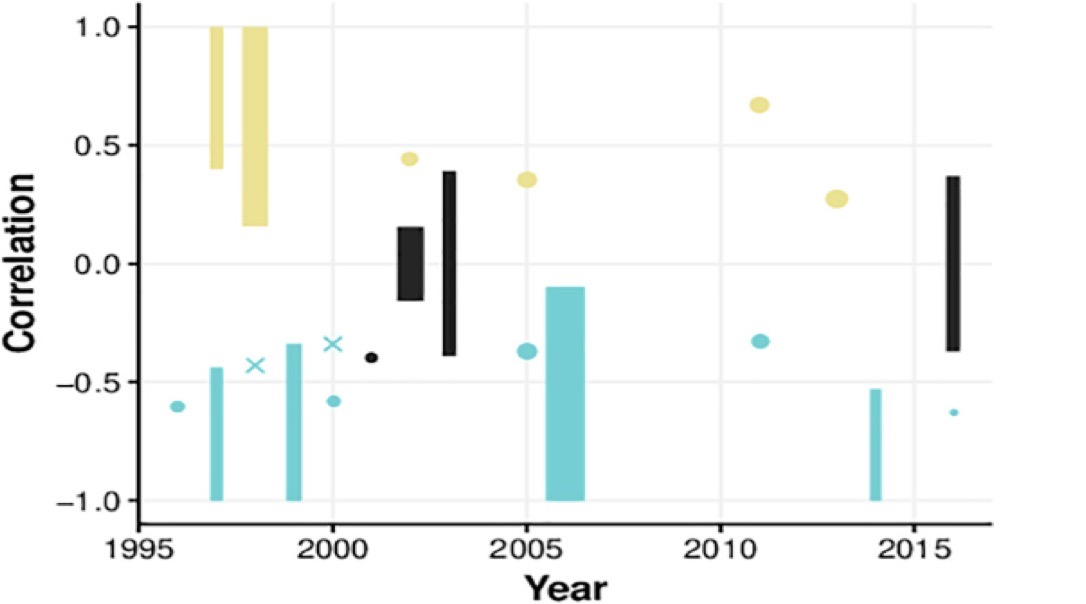
\includegraphics[width=\columnwidth]{presence_vrsick.JPG}
	\caption{Korrelationen von Presence und Cyber Sickness aus der Metaanalyse von Weech et al.\cite{Weech:2019:PresenceCS}. Die Breite der Balken visualisiert die Freiheitsgrade und die Farbe die Signifikanz der Korrelation.}
	\label{abb:presence_vrsick}
\end{figure}

Bei beiden, klassicher Motion und Cyber Sickness, liegt der \textit{visuell-vestibul\"are Konflikt} zu Grunde, jedoch ist die Art, wie dieser entsteht, ebenso wie einige Symptome der beiden, unterschiedlich \cite{Stanney:1997:MSCSSS}. Deswegen wird die Sensory Conflict Theory auch teils als Erkl\"arung f\"ur die Symptome der Virtual Reality Sickness angezweifelt  \cite{Kolasinski:1998:SympCS}. Dennoch l\"asst sich mit ihrer Hilfe gut erkl\"aren, warum die Ma{\ss}nahmen gegen Cyber Sickness in  \autoref{Maßnahmen gegen CS} helfen.

Durch die Symptome kann sich eine Aversion gegen\"uber Virtual Reality entwickeln. Wenn die Teilnehmer das Szenario nicht freiwillig beenden k\"onnen, kann es im Falle von Trainingsszenarien in virtuellen Realit\"aten vorkommen, dass ein unerw\"unschtes Vermeidungsverhalten, wie Passivit\"at, gefestigt wird\cite{Crowley:1987:Avoid}. Dies k\"onnte sich kontraproduktiv auswirken. Daher gilt es sich zu \"uberlegen, mit welchen Mitteln man Virtual Reality Sickness kontrollieren und somit die entstehenden Symptome reduzieren kann, um das gro{\ss}e Potential von Virtual Reality effektiv nutzen zu k\"onnen.


	 
\section{Methoden gegen Cyber Sickness}\label{Maßnahmen gegen CS}
	In diesem Abschnitt sollen verschiedene Ma{\ss}nahmen gegen Cyber Sickness vorgestellt werden. Dar\"uberhinaus soll erkl\"art werden, warum diese wirkungsvoll sind und was m\"ogliche Nachteile bei der Nutzung entsprechender Ma{\ss}nahmen sein k\"onnten.

Die Ma{\ss}nahmen lassen sich in auf Grund der Sensory Conflict Theory in drei Kategorien einteilen: 
Reduktion der Inkongruenz der visuellen Reize entgegen der Erfahrung, indem diese optimiert werden (\autoref{Visuals}), Generation von kongruenten, vestibul\"aren Stimuli entsprechend der Erwartung durch die visuellen Reize (\autoref{Vestibular}) und Adaptation durch den Organismus selbst, unter Beachtung bestimmter Faktoren (\autoref{Adaptation}). Eine generell zu erkennende Tendenz besteht darin, dass diese Methoden versuchen, eine gewohnte \textbf{Nat\"urlichkeit} in der virtuellen Umgebung zu erzeugen.

\subsection{Anpassung der visuellen Reize}\label{Visuals}
Eine Vection passiert dann, wenn ein \textbf{statischer Referenzpunkt} fehlt, an dem man sich optisch fixieren und somit seine Lage relativ dazu sicher feststellen kann. Dies passiert beispielsweise, wenn man aus einem Zug auf einen anderen schaut, ohne den Himmel sehen zu k\"onnen. Wenn der andere Zug sich in Bewegung setzt, erlebt man kurzzeitig Vection, da hier der Himmel als statische Referenz fehlte.

Daher kann ein unabh\"angiger Hintergrund, vorrangig bei CAVE Displays, nach Duh und Parker \cite{Duh:2001:Static} helfen. Nat\"urlich sind die Methoden beispielsweise bei Head-Mounted Displays nicht nutzbar, da diese die visuelle Wahrnehmung der tats\"achlichen Umgebung vollst\"andig ersetzen. Eine Methode dennoch einen bekannten Fixpunkt in die virtuelle Umgebung zu integrieren ist die virtuelle Nase wie in \autoref{abb:vnose}, die laut Wienrich et al.\cite{Wienrich:2018:Nose} die Intensit\"at von Cyber Sickness bei Nutzung von Head-Mounted-Displays reduzieren kann.


\begin{figure}[tbh]
	\centering 
	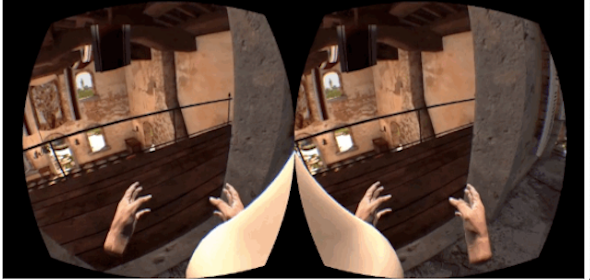
\includegraphics[width=\columnwidth]{virtual_nose.png}
	\caption{Virtuelle Nase zur Reduktion von Cyber Sickness bei Head-Mounted Displays. Bild von WIRED\cite{WIRED:2020:Nose}, letzter Zugriff: 03.05.2020}
	\label{abb:vnose}
\end{figure}


Desweiteren ist es f\"ur die Reduktion von Cyber Sickness ratsam, wenn die graphische Darstellung und Design der virtuellen Umgebung sich dadurch auszeichnen, dass sie nat\"urlich wirken und ruhige, weite Szenen ohne schnellwechselnde Bewegungen nachbildet. Die Parameter der Graphik sollten wie folgt umgesetzt werden:

Die Aufl\"osung und Wiederholungsrate\footnote{50-60 Hz, nach Davis et al.\cite{Davis:2014:Factors}} sollten angemessen hoch sein\cite{kirollos:2019:refresh}, das \textit{Field of View} sollte sich nach Fernandes und Feiner\cite{Fenandes:2016:FOV} dynamisch anpassen und tendenziell eher klein sein und hoch \"uber dem Boden ansetzen, sofern der Kontext, f\"ur den die virtuelle Umgebung genutzt wird, das zul\"asst. Geringe Latenz f\"uhrte nach Meehan et al.\cite{Meehan:2003:latency} zu mehr wahrgenommener Presence und laut Davis et al.\cite{Davis:2014:Factors} auch zu Cyber Sickness, ebenso wie durch Flickern in der Darstellung der virtuellen Umgebung.
Bei all diesen Punkten stellt sich immer die Frage des Aufwandes und der Umsetzbarkeit durch die verf\"ugbare Hardware.

Es scheint, als verursachen realistischere Graphik bzw. Animationen st\"arkere Cyber Sickness\cite{Pouke:2018:Realism}.
In Anbetracht der beiden Punkte, statische Referenz und Nat\"urlichkeit, empfehlen sich weite Landschaften in virtuellen Umgebungen und im Sinne der Sensory Conflict Theory, Fortbewegung in Virtual Reality m\"oglichst zu reduzieren\footnote{In Computerspielen zum Beispiel Teleportation nutzen}, wobei sich hier erneut das Problem ergibt, dass diese Methoden nicht universell einsetzbar sind.

Obwohl mit den genannten Anpassung der visuellen Komponente die Vection schon wesentlich angenehmer und weniger gest\"ort durch Cyber Sickness sein kann, sodass auch eine Immersion in die virtuelle Umgebung stattfindet, ist es immer m\"oglich zus\"atzlich kongruente, vestibul\"are Stimuli zu erzeugen, sodass die Vection keine Illusion mehr ist, sondern nahe an das tats\"achliche Bewegungserlebnis herankommt.


\subsection{Erzeugen kongruenter Stimuli}\label{Vestibular}

Zu den visuellen Reizen der virtuellen Umgebung k\"onnen die verschiedenen Sinneskan\"ale kongruente Stimuli erg\"anzen, auch durch auditive oder haptische, um die Orientierung im virtuellen Raum zu erh\"ohen. Vorrangig l\"asst sich Cyber Sickness aber reduzieren, indem man eine entsprechende M\"oglichkeit der Bewegung einr\"aumt, w\"ahrend man in der virtuellen Umgebung ist. Dies ist vor allem durch sogenannte VRN-Chairs und Treadmills m\"oglich.

VRN-Chairs sind Rollst\"uhle, die mit magnetischen Sensoren ausgestattet werden, sodass die Bewegung der R\"ader des Rollstuhls passend in die Virtual Reality \"ubertragen werden kann. Durch gleichgerichtete Drehung der R\"ader kann eine Vor- oder R\"uckw\"artsbewegung, durch entgegensetzte Drehnung eine Rotation in die jeweilige Richtung erzeugt werden. Durch unterschiedlich starkes Drehen k\"onnen Kurven gefahren werden. Laut Byagowi\cite{Byagowi:2014:VRNchair} reduzieren VRN-Chairs Cyber Sickness und haben den Vorteil, dass sie barrierefrei sind, sodass sie auch in speziellen medizinischen Szenarien genutzt werden k\"onnen. Generell treten im Sitzen in Virtual Reality weniger Symptome von Cyber Sickness auf. Der Nachteil von VRN-Chairs liegt in Anwendungen, welche die dritte Dimension in der virtuellen Umgebung stark beanspruchen.

Eine weitere M\"oglichkeit der Lokomotion in der virtuellen Realit\"at sind Treadmills. Diese sind in der Regel omnidirektional, sodass Bewegung in alle Richtungen m\"oglich ist. Nach Aldaba und Moussavi\cite{Aldaba:2019:VRNTread} sind VRN-Chairs gegen\"uber Treadmills effektiver, da sie den Reizen der nat\"urlichen Bewegung eher entsprechen und dadurch die Symptome der Cyber Sickness weniger intensiv sind, wie in \autoref{abb:comp_vrn_tread} zu sehen ist. Desweiteren beanspruchen Treadmills oft viel Raum. Au{\ss}erdem sind sie gegen\"uber VRN-Chairs nicht barrierefrei und wesentlich kostenintensiver.
\begin{figure}[h]
	\centering 
	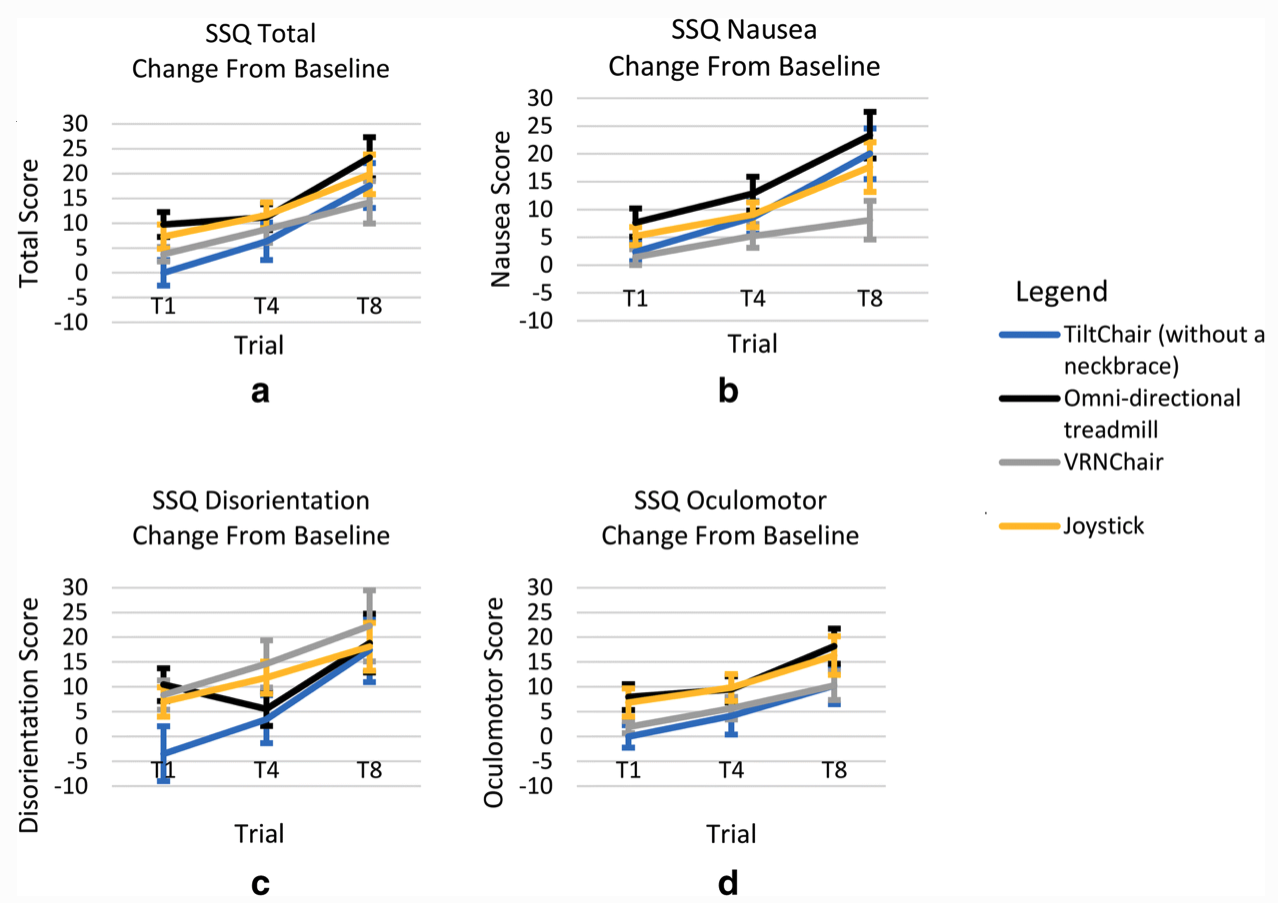
\includegraphics[width=\columnwidth]{comparision_vrn_tread.png}
	\caption{Vergleich verschiederer Methoden bez\"uglich Cyber Sickness von Aldaba und Moussavi\cite{Aldaba:2019:VRNTread}. Niederige SSQ-Scores bedeuten weniger Cyber Sickness.}
	\label{abb:comp_vrn_tread}
\end{figure}

Ohne eine tats\"achlich stattfindende Bewegung, die dann durch die Tr\"agheit der Fl\"ussigkeit in den Bogeng\"angen des Innenohrs einen Reiz erzeugt, funktioniert die \textit{galvanische Vestibul\"arstimulation}, bei der das Gleichgewichtsorgan nicht-invasiv direkt stimuliert wird. Nach Weech et al.\cite{Weech:2020:GVS} kann sie kurzzeitig Cyber Sickness reduzieren, w\"ahrend und kurz nach der Reizung.
Galvanischen Vestibul\"arstimulation scheint effektiv zu sein, weil der Organismus in der virtuellen Umgebung die Gewichtung der Sinneskan\"ale neu bestimmt. Vestibul\"are Reize werden als unzuverl\"assig empfunden und es finden ein \textit{Down-Weighing} statt, wogegen sich mehr auf die visuellen Stimuli verlassen wird und diese st\"arker gewichtet werden.
Der Nachteil dieses Verfahrens ist, dass es noch relativ unerforscht ist und Auswirkungen auf h\"ohere kognitive Schichten unbekannt sind.


Wenn ein Organismus sich nach so kurzer Zeit schon anzupassen beginnt, stellt sich die Frage, wie die Adaptation nach l\"angerer Zeit mit regelm\"a{\ss}iger Nutzung aussieht und welche weiteren Faktoren das Auftreten von Cyber Sickness noch beeinflussen k\"onnen.

\subsection{Adaptation und interindividuelle Faktoren}\label{Adaptation}

Damit eine Anpassung an virtuelle Realit\"aten gelingt, ist es wichtig zu wissen, welche Faktoren \"uber die Inkongruenz der visuellen und vestibul\"aren Stimuli hinaus daf\"ur eine mediierende Rolle haben, sodass man durch die Art und Weise wie und bei wem Virtual Reality genutzt wird, die Adaptation erleichtern kann.

Je l\"anger die sukzessiv verbrachte Zeit in einer virtuellen Realit\"at w\"ahrend einer Session, desto intensiver werden die Symptome der Cyber Sickness\cite{Aldaba:2017:VRNTreadGraphic}, wie auch in \autoref{abb:comp_vrn_tread} deutlich wird. Werden mehr Versuche am St\"uck durchgef\"uhrt werden, so erh\"ohen sich die Scores des SSQ. LaViola\cite{LaViola:2000:CSinVR} konnte zeigen, dass eine Gew\"ohnung an die Virtual Reality stattfindet und sich \"uber mehrere Sessions hinweg so die Cyber Sickness reduziert.

Durch Langzeitpotenzierung ver\"andern sich Neuronen, was als Lernen bezeichnet wird. 
Wie bereits von der galvanischen Vestibul\"arstimulation bekannt ist, kann innerhalb einer Session eine ver\"anderte Verarbeitung der Reize stattfinden, was offenbar auch bleibende Effekte hat. Also lernt man, mit der neuen Situation in der virtuellen Realit\"at umzugehen.
Es empfiehlt sich daher, mit kurzen Sessions zu beginnen und die L\"ange sukzessiv zu erh\"ohen, um dem Organismus Zeit zu geben, sich anzupassen und wenig Belastung durch die Symptome der Cyber Sickness zu verursachen.
Hier muss man sich die Frage stellen, ob der Kontext, in welchem die Virtual Reality genutzt werden soll, genug Zeit f\"ur eine Gew\"ohnungsphase einr\"aumt.

Ein weiterer Faktor ist die Kontrolle, die man in der virtuellen Umgebung hat\cite{Kolasinski:1995:control}. Dies liegt daran, dass sich bestimmte Sinneswahrnehmungen erahnen lassen, wenn man in der virtuellen Umgebung selbst bestimmen kann, was als n\"achstes passiert. Im Sinne der Theorie, dass Motion Sickness einen evolution\"aren Vergiftungsschutz darstellt, ist dieser Faktor sinnvoll. Nervengifte erzeugen nicht nur eine Inkongruenz zwischen den verschiedenen Sinnen, sondern l\"ahmen auch Muskeln, sodass man keine Kontrolle mehr hat. Daher reagiert der K\"orper intensiv, was die Symptome der Cyber Sickness zur Folge hat.

Davis et al.\cite{Davis:2014:Factors} nennen eine Reihe interindividueller Faktoren: Alter, Krankheit, Haltung und Geschlecht. Kinder besitzen danach die h\"ochste Anf\"alligkeit f\"ur Cybersickness, was sich mit zunehmendem Alter reduziert. Die Fl\"ussigkeit der Bogeng\"ange des Innenohrs wird ebenfalls mit zunehmendem Alter viskoser, sodass die vestibul\"areren Stimuli weniger intensiv sind, was wiederum zu weniger Inkongruenz mit den visuellen Reizen f\"uhrt.

Generelle gesundheitliche Probleme, Erkrankungen sowie Alkohol- und Drogenkonsum\cite{Kruk:1992:Drugs} erh\"ohen ebenfalls die Anf\"alligkeit f\"ur Cyber Sickness. Zur Haltung gilt zu sagen, dass Leute mit einer stabileren Haltung weniger unter Cyber Sickness leiden als solche mit einer instabilen. Au{\ss}erdem f\"uhrt Virtual Reality im Sitzen ausgef\"uhrt zu weniger Symptomen als stehend.

Geschlecht gilt als weiterer Faktor. Tendenziell leiden Frauen eher an Cyber Sickness als M\"anner\cite{Aldaba:2019:VRNTread}. Frauen scheinen ein weiteres Field of View zu haben, was Cyber Sickness erh\"oht, wie in \autoref{Vestibular} erkl\"art wurde. Dar\"uberhinaus k\"onnen weibliche Hormone die Anf\"alligkeit erh\"ohen\cite{Kolasinski:1995:control}.


Ein letzter Faktor, der die Adaptation erschweren k\"onnte, ist die Passform des technischen Equipments f\"ur den Anwender, mit dem virtuelle Realit\"aten dargestellt werden - insbesondere bei HMD\footnote{Akronym von Head-Mounted Display}. Der Pupillenabstand bei Menschen folgt einer Normalverteilung, jedoch ist der Abstand bei M\"annern durchschnittlich h\"oher als bei Frauen und die aktuelle Standardgr\"o{\ss}e entspricht im Mittel eher der interpupillaren Distanz bei M\"annern\cite{UploadVR:2020:HMDfit}, sodass die Nutzung im Verh\"altnis f\"ur M\"annern angenehmer ist, ersichtlich in \autoref{abb:hmdfit}. 
\begin{figure}[h]
	\centering 	
	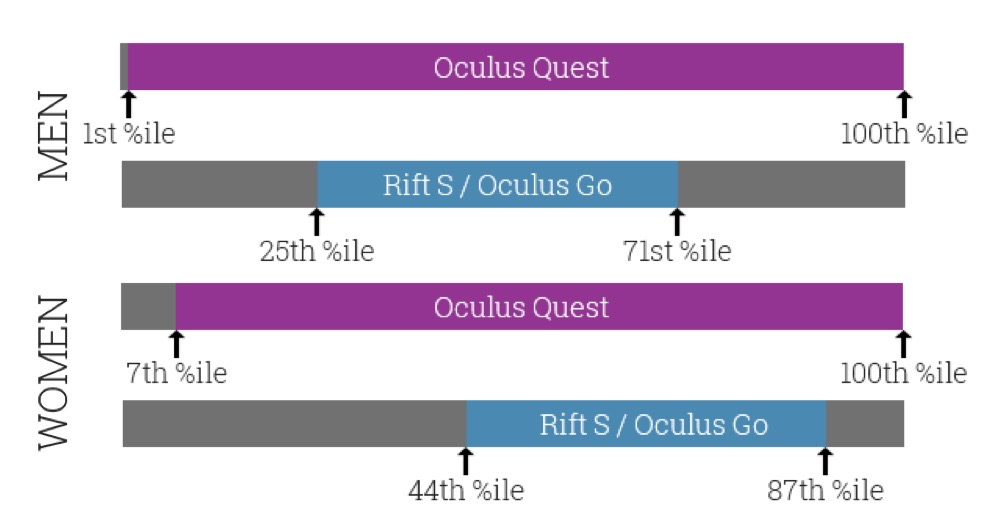
\includegraphics[width=\columnwidth]{fitting.jpeg}
	\caption{Perzentile erwachsener M\"anner und Frauen f\"ur die das jeweilige HMD anhand des Pupillenabstandes am besten geeignet ist. Rift S besitzt einen festen Abstand, im Gegensatz zu Oculus Quest. Bild von UploadVR\cite{UploadVR:2020:HMDfit}, letzter Zugriff: 04.05.2020}
	\label{abb:hmdfit}
\end{figure}


Dieser Faktor k\"onnte auch eine Erkl\"arung f\"ur einige der interindivduelle Faktoren sein, insbesondere Alter und Geschlecht. Da die Erfahrung durch eine schlechte Passform des Head-Mounted Displays f\"ur den Anwender visuell gesehen wesentlich unnat\"urlicher ist, treten Symptome von Cyber Sickness auf.







\section{Fazit}
	Cyber Sickness entsteht durch eine Form des visuell-vestibul\"aren Konflikts und ist, auf Grund der entstehenden Symptome, ein zentraler Aspekt der Nutzung von Virtual Reality. Diese k\"onnen das Erlebnis in einer virtuellen Realit\"at unertr\"aglich machen.

Es wurden in \autoref{Maßnahmen gegen CS} eine Reihe verschiedener Methoden vorgestellt, mit deren Hilfe man, vor allem durch Kombination der Methoden und unter Beachtung bestimmter Faktoren, Cyber Sickness reduzieren kann. Das generelle Prinzip der Nat\"urlichkeit oder Vertrautheit, das es einzuhalten gilt, zieht sich durch die Ma{\ss}nahmen.
Dieses Wissen kann helfen, in Zukunft einen besseren, f\"ur den Anwender angenehmeren Umgang mit weniger Cyber Sickness-Symptomen in Virtual Reality zu erm\"oglichen. Dennoch haben diese Methoden nur bedingte G\"ultigkeit und \"Ubertragbarkeit, da es sich hierbei noch um Grundlagenforschung handelt.

Es ist wichtig zu verstehen, dass momentan keine Theorie existiert, die die Ph\"anomene von Cyber Sickness vollst\"andig erkl\"aren kann. Daher ist es auch nicht m\"oglich zu sagen, ob Cyber Sickness und klassische Motion Sickness denselben Ursprung haben. Dennoch beziehen sich viele Studien \"uber Cyber Sickness in Virtual Reality auf \"altere Studien, in denen es eigentlich um klassische Motion Sickness oder Simulator Sickness geht und versuchen, \"ahnliche Ergebnisse im Sinne der Sensory Conflict Theory zu finden. Dies hat oft widerspr\"uchliche Ergebnisse zur Folge.

Weiterhin folgt aus dieser "`Vererbung"' von der klassischen Motion Sickness an die Cyber Sickness, dass in der Literatur keine eindeutige Nomenklatur herrscht, in der Begriffe wie Cyber Sickness, Virtual Reality Sickness, Simulator Sickness und Motion Sickness teils synonym verwendet werden, ohne dass dies gerechtfertig ist, da es keine genauen Definitionen f\"ur die jeweiligen Begriffe gibt.

Ausgehend von einer exakteren Benennung wird dann zus\"atzliche Forschung ben\"otigt, um eine bessere Theorie zur Erkl\"arung von Cyber Sickness zu finden. Auch m\"ussen neue Messverfahren erschlossen werden, da viele der Messung aktuell auf Selbstausk\"unften beruhen, welche subjektiv verf\"alscht sein k\"onnen. Durch Umsetzen dieser drei Punkte w\"urden danach eindeutigere, weniger widerspr\"uchliche und vor allem besser vergleichbare Ergebnisse entstehen. Es ist wichtig, dies nicht zu vernachl\"assigen, w\"ahrend in der Zwischenzeit mit den aktuellen Gegebenheiten weitergeforscht wird.

Zuletzt sollte bei zuk\"unftiger Forschung und der Umsetzung neuer Methoden an verschiedenste Gruppen gedacht werden, damit keine Ungleichheit zwischen Gruppen herrscht, wie das bei der Passform der Head-Mounted Displays in \autoref{abb:hmdfit} der Fall war. Der Mensch hat sich in seiner Evolution \"uber die Zeit schon an verschiedenste Gegebenheiten angepasst, somit ist anzunehmen, dass selbiges auch f\"ur Virtual Reality gilt. Bis dahin m\"ussen wir uns aber selbst bestm\"oglich unterst\"utzen, durch eben genannte Verbesserung und mit Methoden gegen Cyber Sickness, damit wir das gro{\ss}e Potential, welches Virtual Reality innewohnt, effektiv nutzen k\"onnen.


\section*{Danksagung}{
	Der Autor m\"ochte Amon Ties Uerckwitz f\"ur die Zusammenarbeit im Themengebiet "`Human Factors and Perception"' danken.}


\bibliographystyle{abbrv-doi-hyperref-narrow}
\bibliography{sources}
\end{document}
